\chapter[Summary of Systematic Uncertainties][Summary of Systematic Uncertainties]{Summary of Systematic Uncertainties}
\label{chapter:systematics} 

This chapter summarizes the systematic uncertainties that enter the measurement of the limit of \tth\ multi-lepton analysis. The systematic uncertainties arise from three main sources. The first are the normalization uncertainties on the background process estimation methods, which are discussed in depth in Chapter~\ref{chapter:background}. The second source is the theoretical uncertainties on the \tth\ production cross-section and acceptance. The final source are the experimental and detector related systematic uncertainties related to event selection efficiencies and measurements and identification of the objects. They affect only the non-data driven backgrounds and the \tth\ signal, as simulation is used to model their acceptance and efficiency for the analysis selection. 

These systematic uncertainties, the estimated background and signal event counts in each of the signal regions, and the observed data in each signal region are combined in a statistical fit to an analysis model to extract the measurement of interest. We measure per-channel and combined ratios of the observed production rate to the theoretically predicted production rate of \tth, a parameter called $\mu$. In the absence of a statistically significant observation, this measurement is translated into a upper confidence limit
on $\mu$. The details of this procedure are discussed in the following sections and the results with the observed data are discussed in Chapter \ref{chapter:results}

\section{Systematic Uncertainties on Signal Cross-section and Acceptance}
\label{section:tth}
The \tth\ signal is simulated with matrix elements at NLO in QCD with {\textsc Powhel}. The simulation details are discussed in Chapter \ref{chapter:data}. The production cross section and the Higgs boson decay branching fractions together with their theoretical uncertainties from the QCD scale and PDF choice are taken from the NLO theoretical calculations reported in \cite{Heinemeyer:2013tqa}. The uncertainty from the QCD scale estimated by varying $\mu_{0}$ by a factor of 2 from the nominal value is $^{+3.8\%}_{-9.3\%}$, while the uncertainty from the PDF set and the value of $\alpha_{\rm S}$ is $\pm 8.1\%$.

The impact of the choice of the QCD scale on the simulation of the \ttbar$H$ event selection efficiency is estimated in two independent ways. 

First, the factorization and renormalisation scales $\mu_{0}$ are varied by a factor of 2, as $\mu = 2\mu_{0}$ and $\mu = \mu_{0}/2$. The effects of these new scales are estimated via the application of event re-weighting procedures on the nominal simulation using kinematic distributions at parton level. The weights used are dependent on the transverse momenta of both the \ttbar$H$ system and of the top quark, as described in \cite{Guindon:1638000}. 

Second, the choice of the factorization and renormalisation scales, dependent on fixed (static) parameters in the nominal simulation, is tested comparing its prediction with an alternative (dynamic), but still physics motivated choice $\mu_{0} = (m_{T}^{t}m_{T}^{\bar{t}}m_{T}^{H})^{\frac{1}{3}}$, which depends on kinematic variables. This comparison is performed via event re-weighting of the nominal static simulation based on weights derived as a function of the \ttbar$H$ transverse momentum~\cite{Guindon:1638000}. In order to take the difference between the choices of scale as systematic uncertainties, a symmetric envelope around the nominal simulation is built applying the weights and also their inverses.

In order to not double-count the variations on the total cross section the predictions from the different QCD scales are normalized to the same total cross section. That means that the observed differences are only coming from the event selection.
Significant variations on the jet multiplicities can be seen and these translate into different predictions on the signal event yields in the signal regions. Such differences, listed in Table~\ref{table:systematics_theosystttH}, are taken as theoretical systematic uncertainties in addition to the ones affecting the total \ttbar$H$ production cross section. The static uncertainties come from the variations by a factor of 2 from the nominal scale and they are correlated with the uncertainties on the total cross section, which are estimated with the same procedure. The dynamic uncertainties come from the difference between the nominal and the alternative dynamic scale and are treated as an independent source of theoretical uncertainty. 

\begin{table}
\caption{Theoretical uncertainties of the signal event yields in the signal regions due to the impact of QCD scale uncertainties on the event selection.}
\begin{center} 
\begin{tabular}{r|c|c|c|c|}
QCD scale [\%] & 2$\ell$4jets & 2$\ell$$\geq$5jets & 3$\ell$ & 4$\ell$ \\
\hline
Static   & $^{+0.6}_{-0.0}$ & $^{+2.7}_{-1.3}$ & $^{+2.3}_{-0.8}$ & $^{+0.9}_{-0.2}$ \\
Dynamic  & $^{+1.7}_{-0.8}$ & $^{+2.0}_{-2.6}$ & $^{+1.7}_{-1.1}$ & $^{+0.5}_{-0.0}$ \\
\hline
\end{tabular}
\end{center}
\label{table:systematics_theosystttH}
\end{table}%

The uncertainty of the \ttbar$H$ event selection due to the PDF sets is estimated comparing the predictions with three different PDF sets, varying each set within errors and taking the width of the envelope as systematic uncertainty. The recommended sets are \verb+CT10+, \verb+MSTW2008nlo68cl+ and \verb+NNPDF21_100+. 

Figure~\ref{figure:systematics_theosystPDF} shows the estimated PDF systematic uncertainties as a function of the jet multiplicity in \ttbar$H$ events with at least two leptons. The uncertainties are compatible with the uncertainty on the production cross section estimated in \cite{Heinemeyer:2013tqa} and indicated by the dashed red lines in the lower panel. 
Table \ref{table:systematics_pdfaccttH} shows the half-width of the envelope of the acceptance under all eigenvector variations of the three PDF sets.
No significant dependence on the event topology is observed, so that the PDF systematic uncertainty on the \ttbar$H$ event selection is neglected.
\begin{figure}[htbp]
\begin{center}
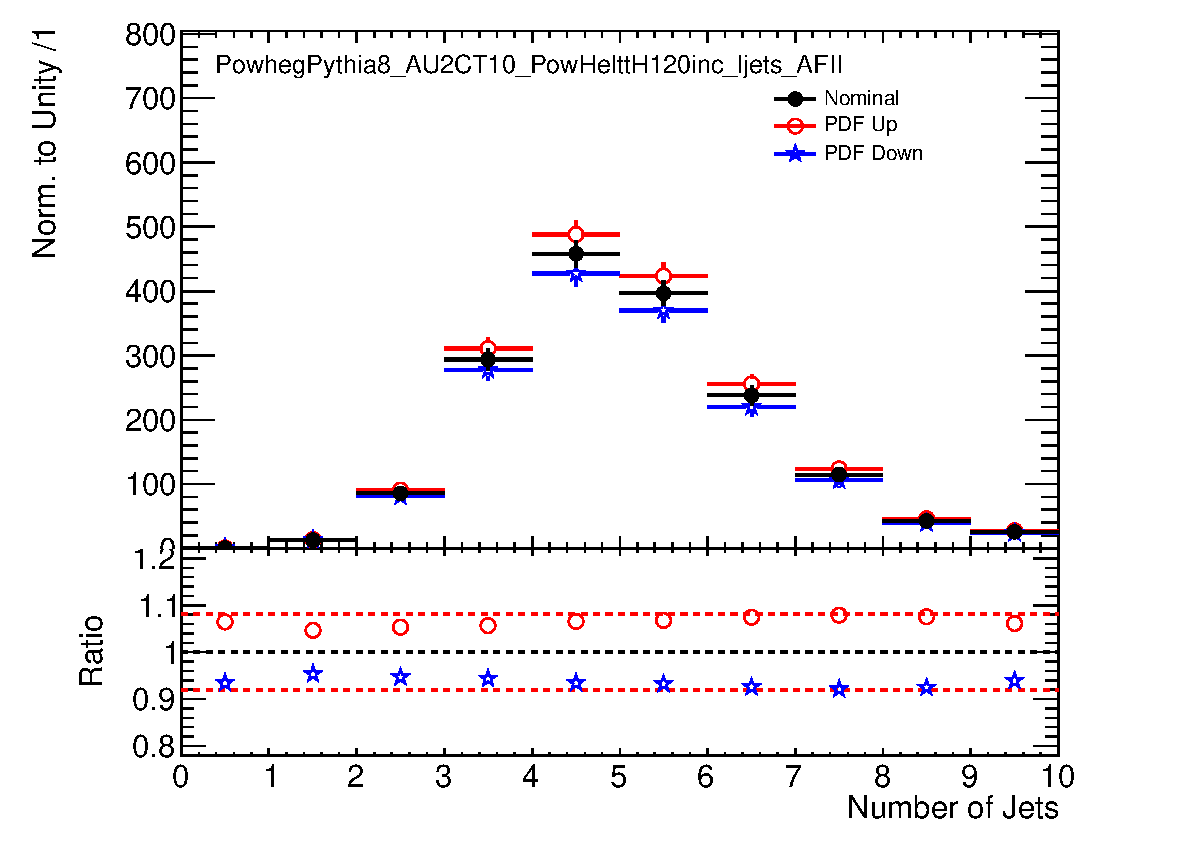
\includegraphics[width=0.6\textwidth]{figs/tth/plot_PowhegPythia8_AU2CT10_PowHelttH120inc_ljets_AFII_njets_all_njets_all}
\caption{PDF systematic uncertainty on the jet multiplicities in \ttbar$H$ events with at least 2 leptons. The dashed red lines in the lower panel indicate the systematic uncertainty on the \ttbar$H$ production cross section.}
\label{figure:systematics_theosystPDF}
\end{center}
\end{figure}

\begin{table}
\begin{center}
\caption{\label{table:systematics_pdfaccttH}Uncertainties on $\ttbar H$ acceptance in signal
  regions due to PDF variation.}
\begin{tabular}{r|c|c|c|c}
Sample & 2$\ell$ 4j & 2$\ell$ 5j & 3$\ell$ & 4$\ell$\\
\hline
$\ttbar H$ & 0.3\% & 1.0\% & 0.5\% & 1.4\%\\
\end{tabular}
\end{center}
\end{table}

The acceptance uncertainty related to the parton shower and underlying event modelling is estimated by comparing the event yields in the signal regions with the nominal
parton shower and underlying event generator ({\textsc PYTHIA}) with {\textsc HERWIG$++$}. The statistical uncertainties on these comparison are larger than any observable
systematic effects but are still small compared to the above uncertainties (1-3\%). 


\section{Experimental and Detector Systematic Uncertainties}
 
Experimental and detector systematic uncertainties affect the efficiencies of identifying objects and the efficiencies for events to pass our cuts . These uncertaintites affect only MC models of physics processes, \ttV, \tth, $VV$ and thus alter ther number of expected events from signal and backgroun in our signal regions. Data-driven backgrounds take into account these uncertainties by construction. We consider systematic effects from a number of sources: the lepton and jet energy scale measurements, the lepton identification and isolation selections, the efficiency and misidentification rate associated with tagging b-quark jets. Effects due to modeling the energy and objects from additional vertices were studied and found to be negligible. The vast majority of the individual detector systematics effects are small. The sum total of the systematic effects are comparable to the overall normalization and cross-section uncertainties on some of the physics processes and is shown in Table \ref{table:systematics_total_detector}.

\subsection{Lepton Identification, Energy Scale, and Trigger}
The electron\cite{ATLAS-CONF-2014-032} and muon identification efficiencies\cite{MuonSF} are measured in data using $Z$ boson and $J/\Psi$ control samples. They muon efficiencies are shown in Figure \ref{figure:systematics_lepidsf}, while the lectron efficienceis are shown in Figure~\ref{figure:electron_eff}. The uncertainty on the muon efficiencies are measured as functions of $\eta$ and \pt\ and are generally less 1\%. The uncertainty on the electron and muon efficiencies are also measured as functions of $\eta$ and \pt\ and are at the 1\% level for \pt\ above 30 GeV, but become much larger 5-10\% for the lower \pt\ regimes.   These translate into sub-1\% level effects on the \ttV\ and \tth\ event counts in the signal regions for the muons and 1\% level effects for the electrons. The effects become more important with increasing numbers of leptons.  

\begin{figure}[htbp]
\begin{center}
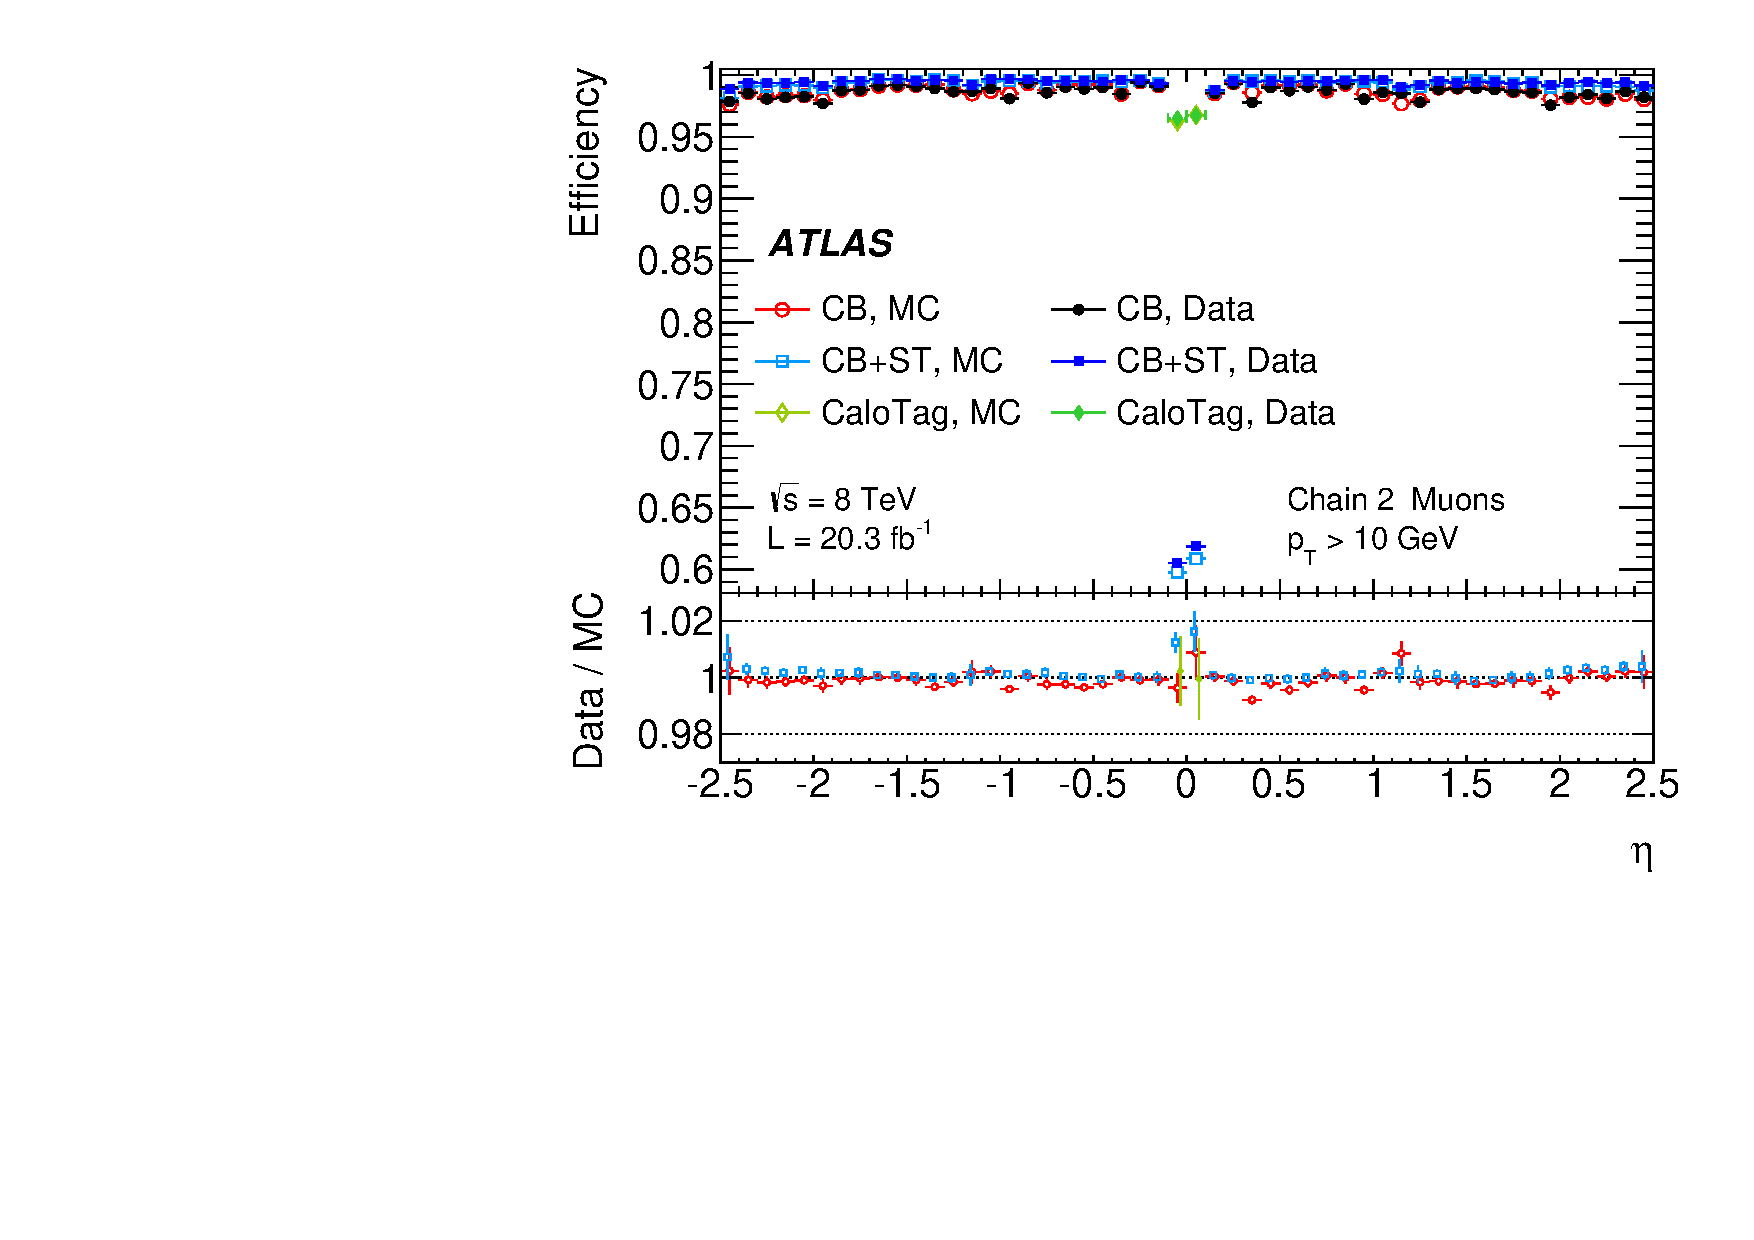
\includegraphics[width=0.60\textwidth]{figs/systematics/fig_18a}
\caption{Muon identification efficiency in Data and MC as a function of $\eta$. The CB+ST (combined+segment tagged) operating point is used}
\label{figure:systematics_lepidsf}
\end{center}
\end{figure}

The electron\cite{EgammaReco} and muon\cite{MuonSF} energy scale and resolution are also measured using the $Z$-boson control samples in data. The uncertainties related to the scale and resolution for the leptons affect the overall event acceptance through the lepton momentum cuts primary and have negligible impact on the event count uncertainties in the signal regions.

The efficiencies for muons and electrons to pass muon\cite{ATLAS-CONF-2012-099} and electron triggers\cite{ATLAS-CONF-2012-048} have been calculated with respect to the offline identification operating points using the $Z$ boson control samples. They are in the range of 90\% for electron triggers and 70\% for muon triggers, owing to gaps in muon trigger coverage, and have 1\% level uncertainties. When statistically combined for 2$\ell$ SS, 3$\ell$ and 4$\ell$ lepton signal regions, the overall trigger efficiency is high and the uncertainties on the number of expected events is negligible. 


\subsection{Lepton Isolation and Impact Parameter}

The isolation and impact parameter selections are specific to this analysis and are discussed in depth in Chapter \ref{chapter:selection}. We calculated their combined efficiency with respect to the full lepton identification selection using the $Z$ boson control samples and define data-MC scale factors to correct the efficiency in the simulation. Background are subtracted using shape templates in the di-lepton invariant mass spectrum. The $Z$-event template is derived from MC, while the background template is derived from the same-sign control region. We measure the efficiency scale-factors in bins of lepton momentum. Uncertainties are assigned per-bin to account for the level of statistics and variations caused by the fit parameters. An additional 1\% uncertainty envelope is added to both the electron and muon measurements to account for trends observed in the dependence of the data-MC efficiency scale-factor as a function of the number of jets. Stability of the efficiency scale-factor as a function of the number of jets is important for this analysis, because event activity in the low jet $Z$ sample, where the efficiency is measured, is much different from the high jet signal regions, where the efficiency is applied. The dependence of the scale-factor on the number of jets can be seen Figure \ref{figure:systematics_iso}. The isolation scale-factor uncertainties are around 1-3\% depending on the particle momentum, but these uncertainties propagate to 2-5 \% (some of the largest) effects in the event counts in the signal regions. The uncertainties are more important in the regions with more leptons. 


\begin{figure}[htbp]
\begin{center}
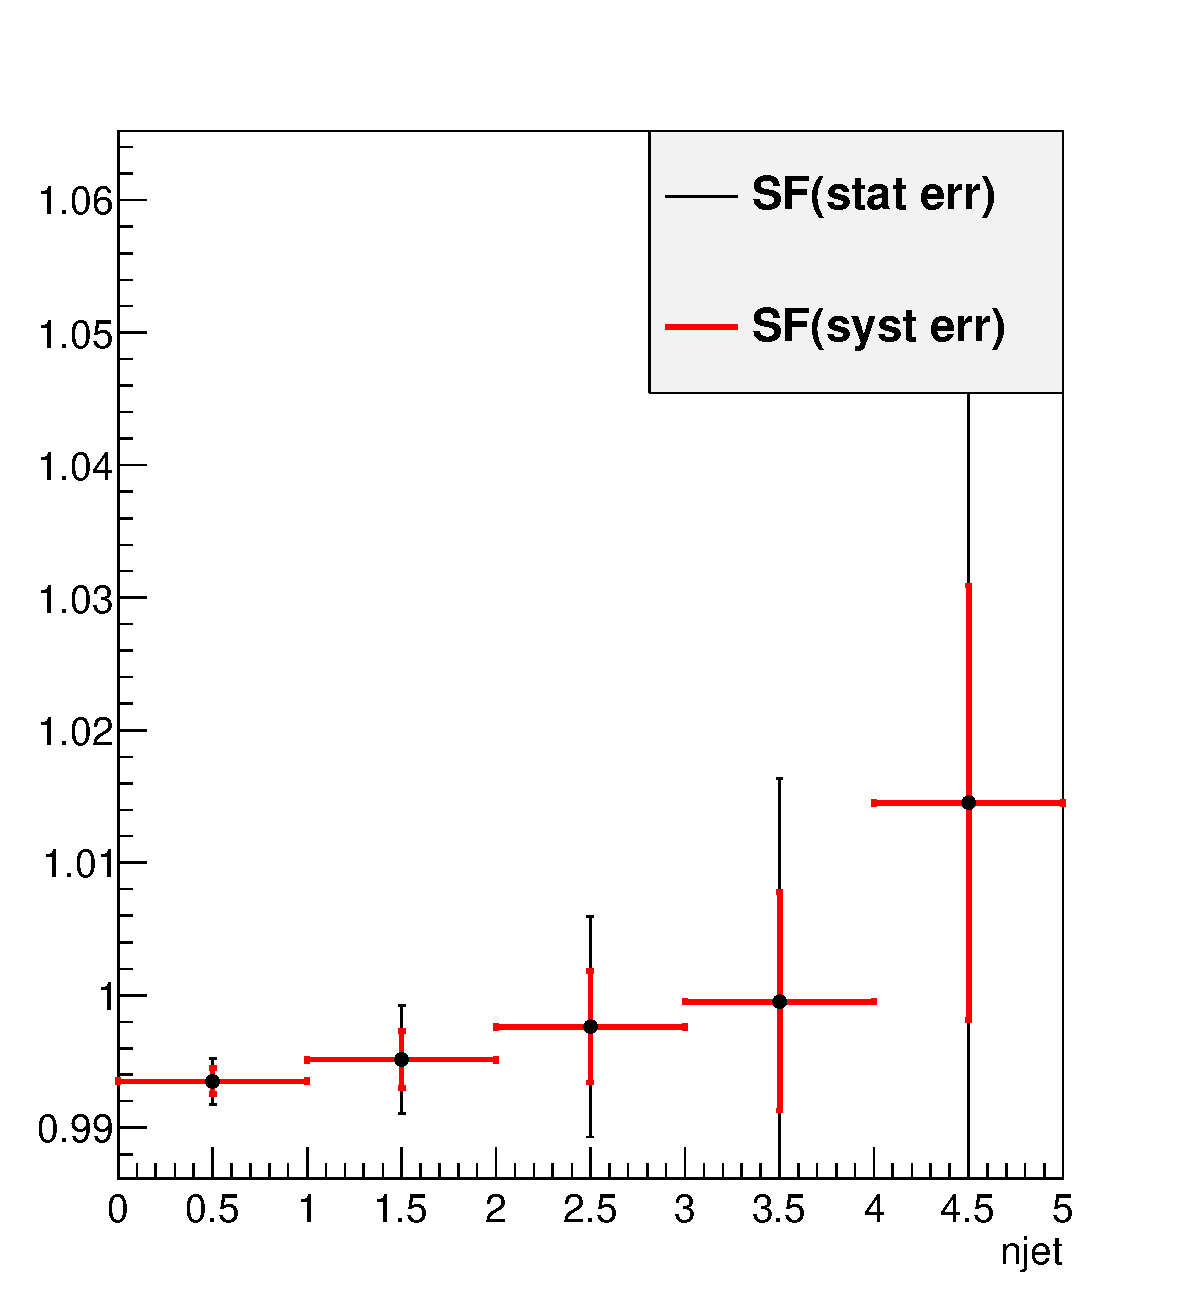
\includegraphics[width=0.48\textwidth]{figs/systematics/MuTP_sf_njet_ALP}
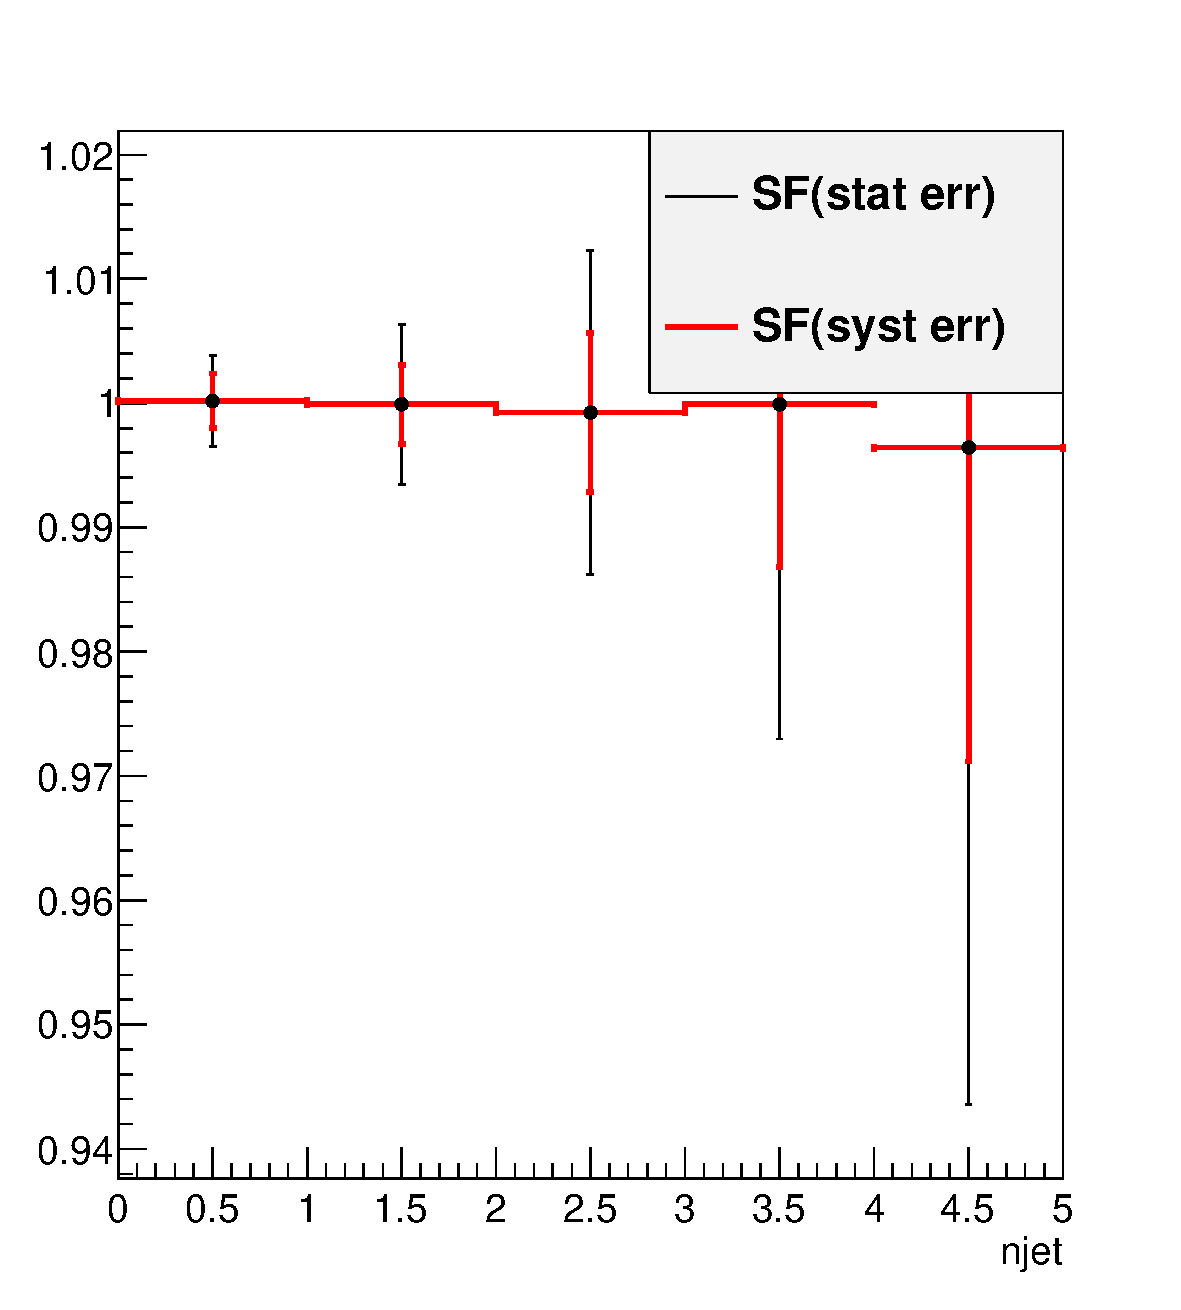
\includegraphics[width=0.48\textwidth]{figs/systematics/EleTP_sf_njet_ALP}
\caption{Muon (left) and electron(right) isolation efficiency scale-factors from the $Z$ control sample as a function of the number of jets in the event. An additional systematic uncertainty of 1\% is added to encompass the variation in the number of jets variable}
\label{figure:systematics_iso}
\end{center}
\end{figure}


\subsection{Jet Energy}

The jet energy scale (JES) is calculated using a combination of data-based in-situ techniques, where jet transverse momentum is balanced with respect to a reference photon or a Z boson, as well as single particle test-stand studies\cite{Aad:2014bia}. Additional smaller effects are taken into account including the b-quark jet specific response, near-by jets, the effects of pile-up and an inter-calibration of similar $\eta$ regions using di-jet events. These effects are measured in 2012 data. The JES systematic errors arises from numerous sources that are diagonalized into eigenvectors so that they can be combined in an uncorrelated way. The combined uncertainty is plotted in Figure \ref{figure:systematics_jes} as a function of jet $\eta$ and \pt\ and is the range 2-4\% for jets used in this analysis. The jet energy resolution is calculated in a similar way with slightly larger errors, 10\% \cite{Aad:2012ag}. The combined scale and resolution systematics are of non-negligible effects 6-7\% on the signal and background event counts in the signal regions.  


\begin{figure}[htbp]
\begin{center}
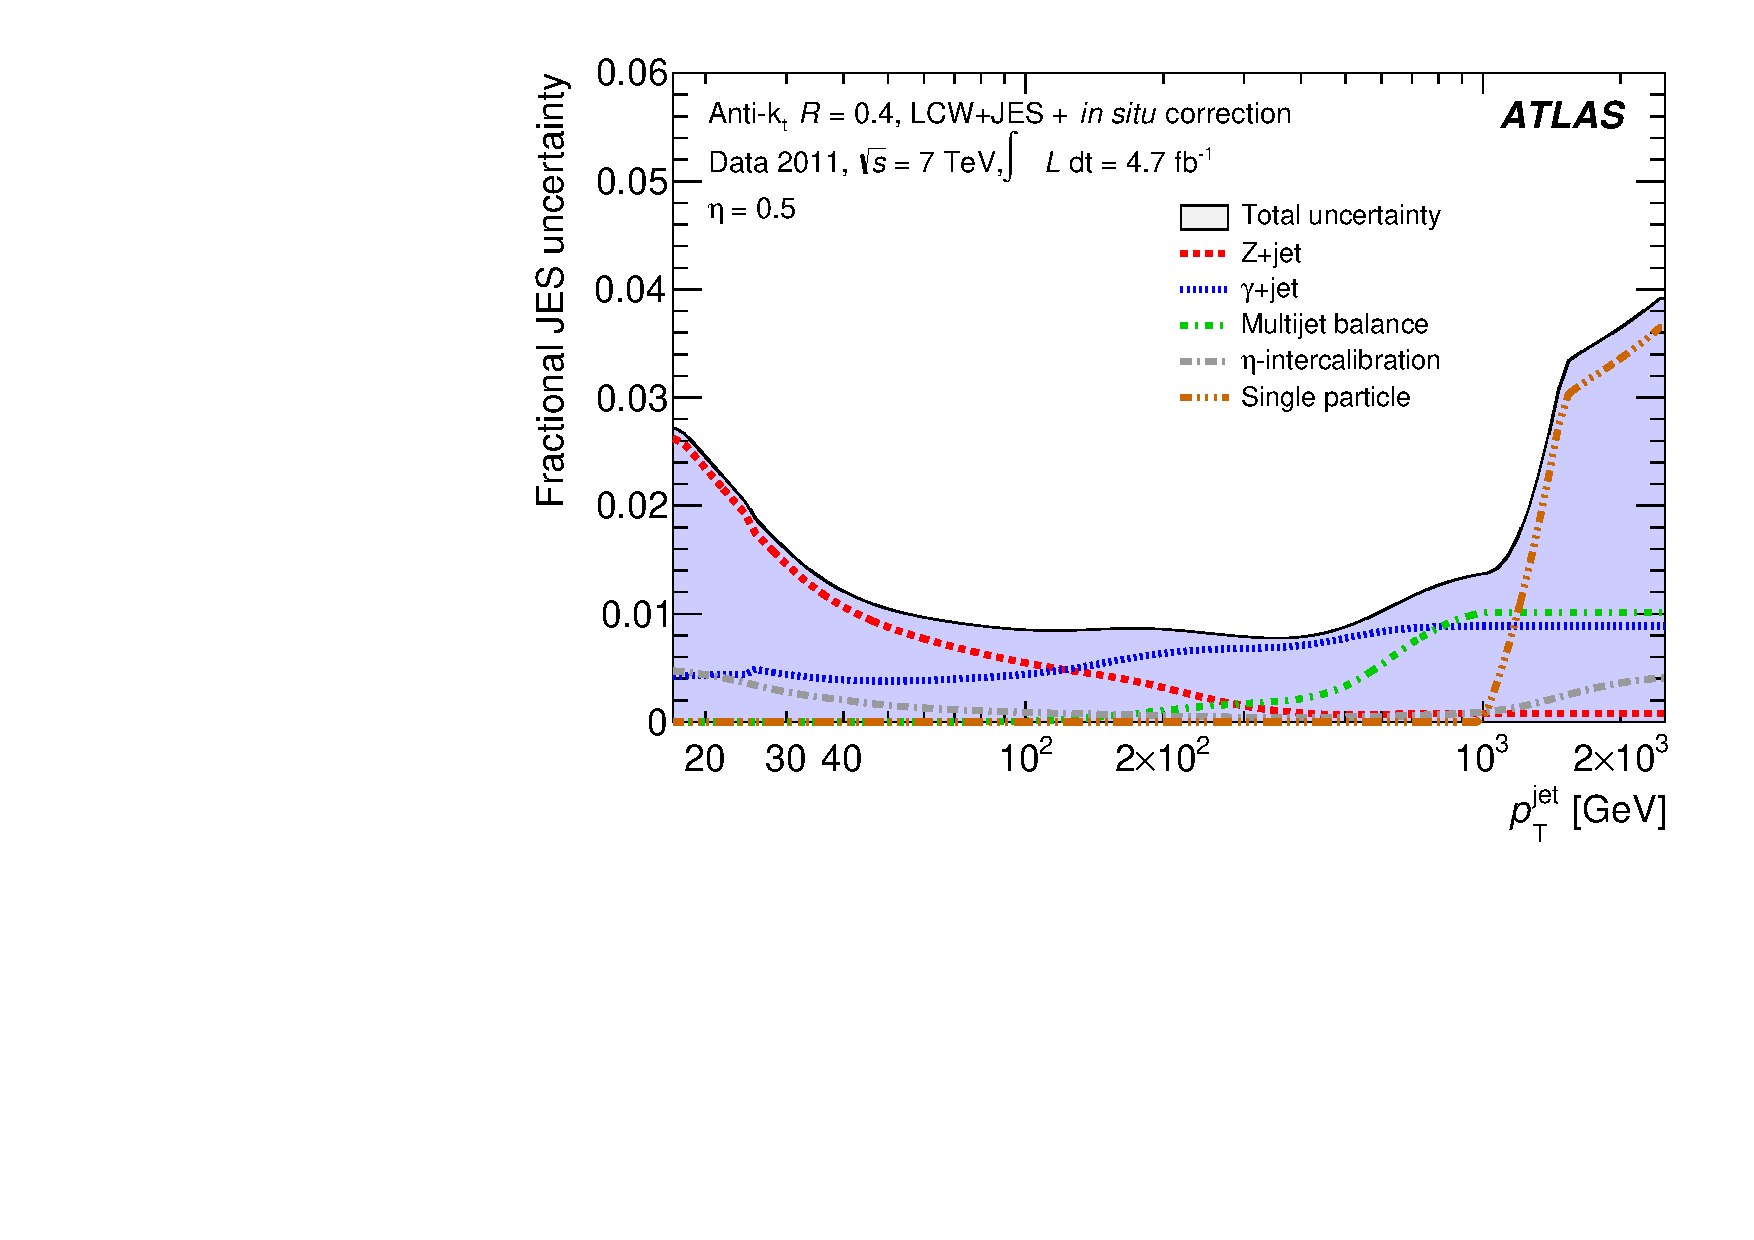
\includegraphics[width=0.48\textwidth]{figs/systematics/fig_61a}
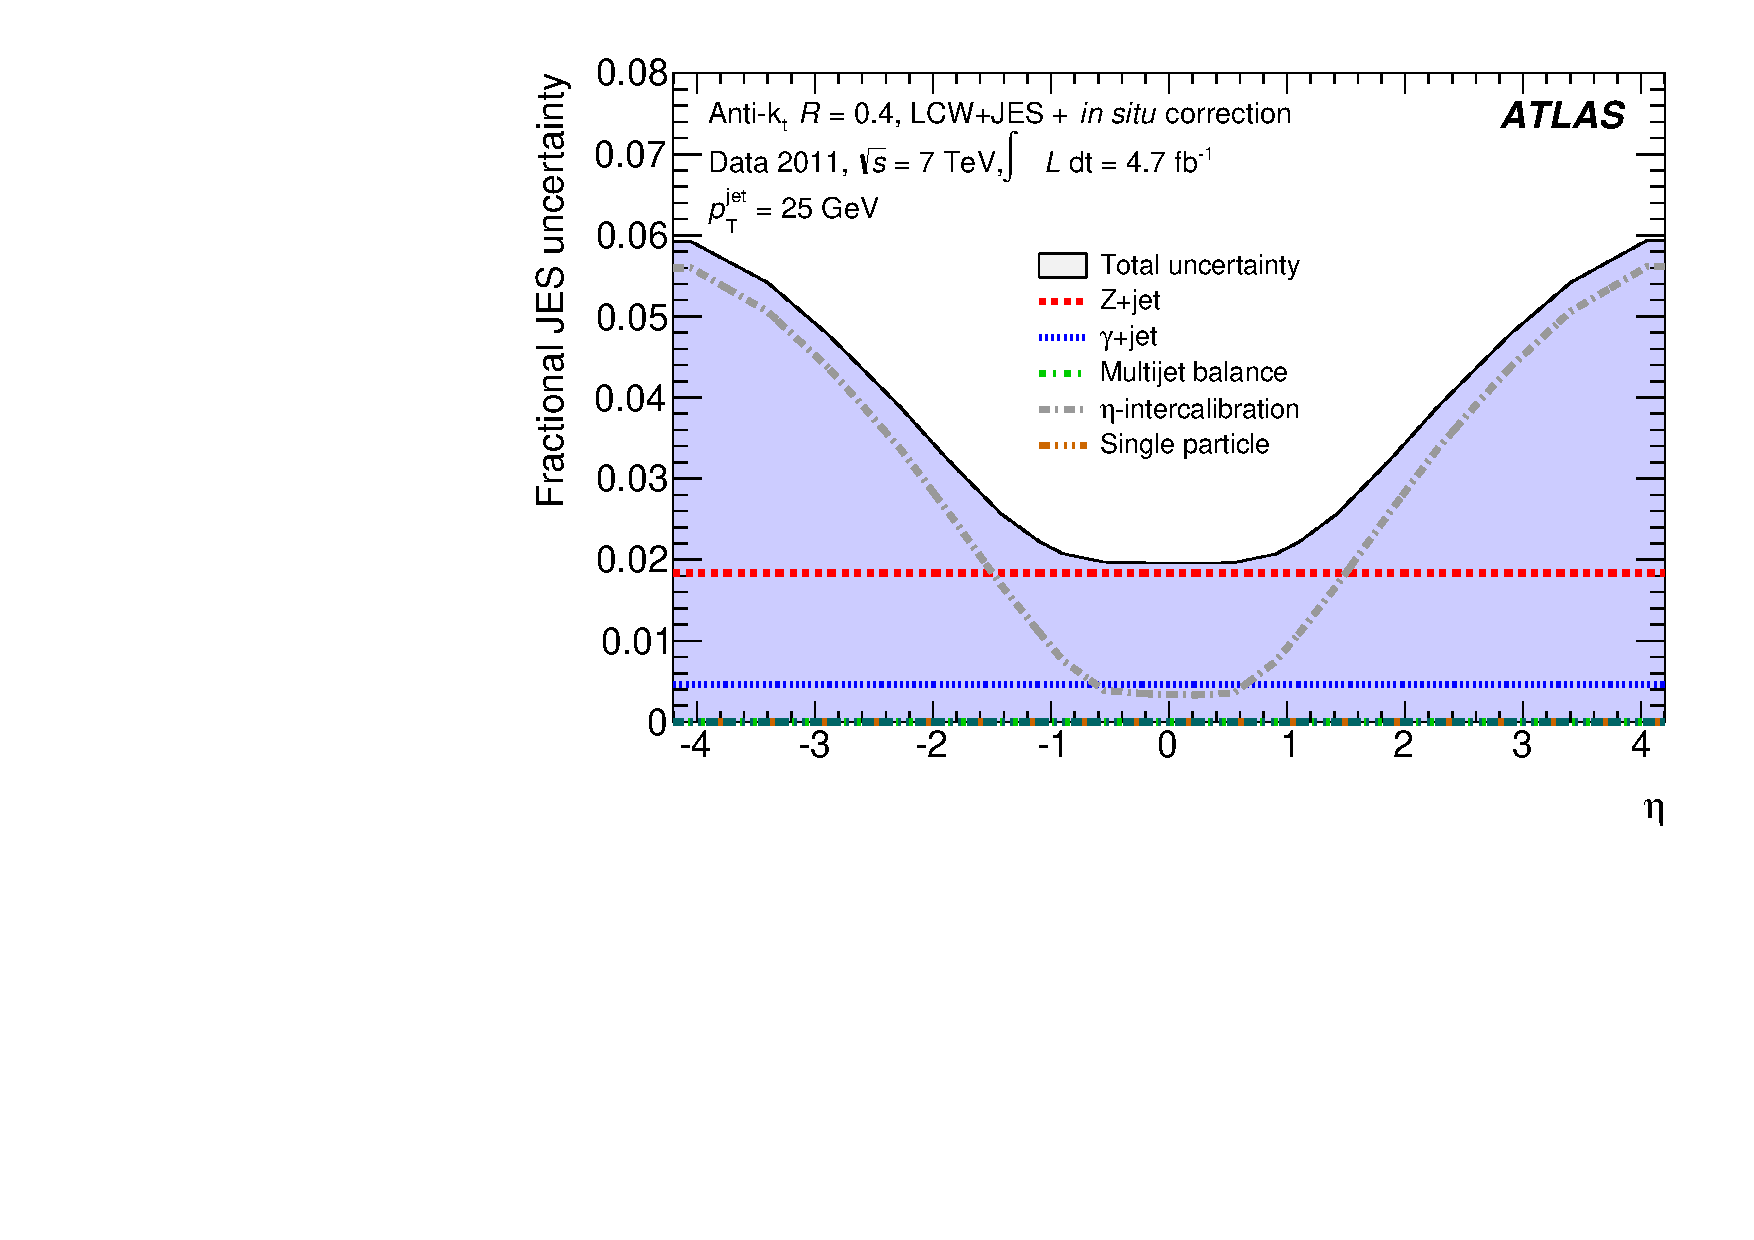
\includegraphics[width=0.48\textwidth]{figs/systematics/fig_61c}
\caption{JES systematic uncertainties as a function of jet $\eta$ (for jets \pt $>$ 25 GeV) and \pt\ (for jets $|\eta|<0.4$). The combined systematic uncertainty is shown with contributions from the largest sources}
\label{figure:systematics_jes}
\end{center}
\end{figure}


\subsection{B-Tagged Jet Efficiency}

The $b$-quark tagging efficiency must be calculated separately for charm, light and b-quarks. ATLAS uses three data based control regions: an inclusive jet sample for mistagged light quarks\cite{mistagratecalibration}, the \ttbar\ sample for b-quarks\cite{bjetcalibration}, and a sample of $D^{*}$ mesons for charm quarks\cite{cjetcalibration}. These efficiencies and rates are well-measured in MC and the data-based corrections are small. The data-MC efficiency scale-factor shown in Figure \ref{figure:systematics_b} is close to 1 and has an overall systematic uncertainty of around 5\%. The uncertainties are applied to the analysis via a number of eigenvectors. Together these uncertainties have a 4 \% effect in the event expectation in the signal regions. 

\begin{figure}[htbp]
\begin{center}
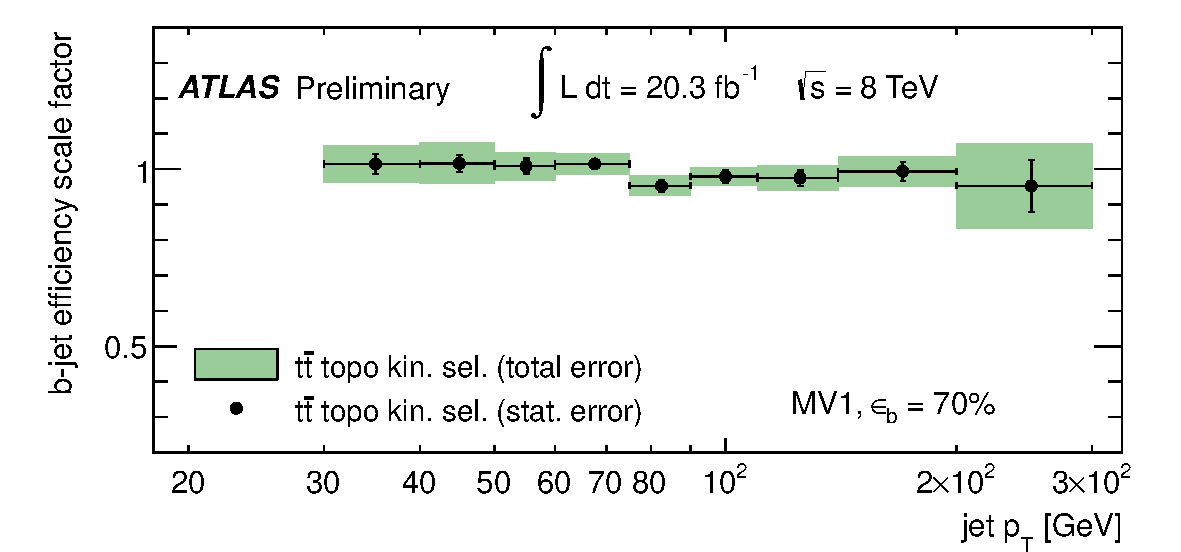
\includegraphics[width=0.48\textwidth]{figs/systematics/ttbartopo}
\caption{b-Tagging data-MC efficiency scale-factors versus jet \pt\ calculated in the \ttbar\ sample from 2012 data. The uncertainties are combined statistical and systematic.} 
\label{figure:systematics_b}
\end{center}
\end{figure}


\subsection{Summary}

The combined effect of these detector and experimental systematics on the \ttV\ and \tth\ is provided in Table \ref{table:systematics_total_detector}. The effects are smaller than the normalization uncertainties on some of the backgrounds. They are dominated by the lepton isolation scale-factor measurements and the electron identification with smaller contributions from the JES and b-tagging efficiencies. These detector systematic uncertainties enter the fit individually and the most important to the overall measurement uncertainty can be seen in Figure~\ref{figure:results_nuisance}.

\begin{table}
\begin{center}
\begin{tabular}{r|cc|cc|cc|cc|}
Total Systematic & \multicolumn{2}{c|}{2ee4j} & \multicolumn{2}{c|}{2ee5jincl} & \multicolumn{2}{c|}{2em4j} & \multicolumn{2}{c|}{2em5jincl} \\ 
Uncertainty & \multicolumn{2}{c|}{Down-Up} & \multicolumn{2}{c|}{Down-Up} & \multicolumn{2}{c|}{Down-Up} & \multicolumn{2}{c|}{Down-Up} \\ 
\hline 
ttH & -4.68 & 5.84 & -8.24 & 6.14 & -5.10 & 3.50 & -5.52 & 6.40   \\ 
ttW & -7.20 & 5.45 & -8.72 & 11.30 & -3.63 & 6.22 & -9.72 & 7.95 \\ 
ttZ & -9.68 & 5.07 & -5.87 & 10.98 & -4.07 & 6.16 & -8.37 & 4.99 \\ 
\hline 
Total Systematic & \multicolumn{2}{c|}{2mm4j}& \multicolumn{2}{c|}{2mm5jincl} & \multicolumn{2}{c|}{3$\ell$} & \multicolumn{2}{c|}{4$\ell$} \\ 
Uncertainty & \multicolumn{2}{c|}{Down-Up} &\multicolumn{2}{c|}{Down-Up} & \multicolumn{2}{c|}{Down-Up} & \multicolumn{2}{c|}{Down-Up} \\ 
\hline 
ttH &-5.20 & 7.51& -7.28 & 6.75 & -5.84 & 5.59 & -6.54 & 6.54\\ 
ttW &-4.54 & 5.23& -8.63 & 6.88 &  6.36 & 8.16 & --- & --- \\ 
ttZ &-5.24 & 8.69& -9.73 & 8.18 & -6.14 & 6.66 & -9.58 & 6.94\\ 
\end{tabular} 
\caption{Sum in quadrature of all the systematic uncertainties on the number of event yields per channel.}
\label{table:systematics_total_detector} 
\end{center} 
\end{table} 


\section{Summary of Background and Signal Normalization Uncertainties}

Table \ref{table:systematics_summary} gives the summary of the systematic uncertainties that are included in the analysis for the normalization and acceptance of each process. The relative importance of these uncertainties to the final fit can be seen in Figure~\ref{figure:results_nuisance}.  


\begin{table}[htbp]
  \begin{center}
    {\small     
    \begin{tabular}{|lll|}
      \hline
      Type       & Description  &  Uncertainty  \\
     \hline
      \multicolumn{3}{|c|}{Signal (ttH)}\\
     \hline
         &  &                \\
      QCD Scale                    & Cross Section (Dynamic Scale) &    $+3.8\%$  $-9.3\%$   (Section~\ref{section:tth})      \\
                                            & Analyses Acceptance          &    $0.$-$2.6\%$       \\
         & &                \\
      PDF+$\alpha_S$     &   Cross Section  &         $\pm$ 8.1$\%$      \\
                                      &   Analyses Acceptance        &     $0.3$-$1.0\%$        \\

         & &                \\
      Parton Shower     &   Analyses Acceptance  &        $0.2$-$1.4\%$       \\
         & &                \\
     \hline
      \multicolumn{3}{|c|}{ttW (Irreducible background)}\\
     \hline
         & &                \\
      QCD Scale                    & Cross Section (Dynamic Scale)  &    $\pm15\%$  (Section~\ref{section:ttV} )       \\
                                            & Analyses Acceptance   &    $0.4$-$3.5\%$        \\
         & &                \\
      PDF+$\alpha_S$     &   Cross Section  &         $\pm$ 13$\%$      \\
                                      &   Analyses Acceptance  &        $1.1$-$4.8\%$      \\
      
         & &                \\
      Matching          &   Analyses Acceptance  &        $0.2$-$10.\%$       \\
      Modelling         &   Analyses Acceptance  &        $0.1$-$15.6\%$       \\
      Parton Shower     &   Analyses Acceptance  &        $2.4$-$13.0\%$       \\
         & &                 \\
     \hline
      \multicolumn{3}{|c|}{ttZ (Irreducible background)}\\
     \hline
         &  &                 \\
      QCD Scale                    & Cross Section (Dynamic Scale)     &    $\pm12\%$     (Section~\ref{section:ttV})\\
                                            & Analyses Acceptance              &    $0.1$-$3.1\%$          \\
         & &                 \\
      PDF+$\alpha_S$     &   Cross Section  &         $\pm$ 9$\%$       \\
                                      &   Analyses Acceptance          &     $0.9$-$2.7\%$      \\
      
         & &                \\
      Matching          &   Analyses Acceptance  &        $0.5$-$16.\%$       \\
      Modelling         &   Analyses Acceptance  &        $3.5$-$10.5\%$       \\
      Parton Shower     &   Analyses Acceptance  &        $2.4$-$13.0\%$       \\
         & &                 \\
     \hline
      \multicolumn{3}{|c|}{VV Backgrounds}\\
     \hline
         &   &              \\
      Normalization Uncertainty             &   \WZ,ZZ Processes       &         $\pm$ 50$\%$   (Section~\ref{section:wz})   \\
          &  &             \\
     \hline
      \multicolumn{3}{|c|}{Data-Driven Backgrounds}\\
     \hline
          &   &             \\
           Normalization Uncertainty                 &    Jet Fakes       &     $\pm$ 30-50$\%$ (Section~\ref{section:fakes})     \\
           Normalization Uncertainty                 &    Charge MisID    &     $\pm$ 30-40$\%$ (Section~\ref{section:qmis})      \\
          &    &             \\
     \hline
    \end{tabular}
    }
    \caption{ Summary of systematic uncertainties for processes present in the signal regions in the analysis, with their
    type, description, name, values and uncertainties, and status of inclusion in the final results.}
    \label{table:systematics_summary}
    \end{center}
    \end{table} 


